\chapter{Predchádzajúce riešenia}

\section{Verifikačný softvér}

Verifikácia predpovedných modelov počasia je úloha dokonale stvorená pre automatizáciu. 
Z tohto dôvodu meteorológovia začali využívať dostupný štatistický softvér 
a neskôr boli taktiež vyvíjané špecializované nástroje určené pre verifikáciu.
Môžeme teda rozdeliť verifikačný softvér do dvoch základných kategórií a to \textit{štatistický} a \textit{špecializovaný}, ktorý je zväčša podporovaný rôznymi národnými a medzinárodnými organizáciami.

\subsection{Štatistický softvér}
%TODO
Spoločnou črtou: \\
	- obmedzená funkcionalita \\
	- obmedzená vizualizácia \\
	- slabé / žiadne GUI \\
	- vyžaduje znalosť špecifického programovacieho jazyka \\
	- ...


\subsubsection{Tabuľkový softvér}
Napriek tomu, že je tabuľkový softvér na výpočet štatistík zamietnutý komunitou vedcov a štatistikov ako nevhodný a neprofesionálny, tak je využívaný, a to pomerne často, aj vo vedeckých kruhoch. 
Výhodou je, že novému užívateľovi umožňuje okamžite vidieť všetky kroky v základných procedúrach verifikácie a teda je výborný pre výučbové účely. \cite{VerifSoft} 
Najznámejší kus softvéru z pomedzi komerčných produktov je \textit{Microsoft Excel} \cite{Excel} a z voľne dostupných je jeho opensoruce náprotivok \textit{Open Office Calculate} \cite{OpenOfficeCalc}. Oba programy zahrňujú základné štatistické funkcie ako napríklad stredná kvadratická chyba (\textit{MSE}) pre spojité predpovede (pozri odsek \ref{subsec:mse}) a taktiež umožňujú generovanie jednoduchých grafov na základe tabuľkových dát. Tabuľkový softvér neposkytuje priamo funkcionalitu na výpočet ďalších sofistikovanejších verifikačných štatistík, avšak umožňuje ich implementáciu pomocou makro programovania v špecifickom jazyku. Pre Microsoft Excel je to \textit{Microsoft Visual Basic for Applications}(VBA) \cite{VBA} a pre Open Office Calculate zasa \textit{OpenOffice.org Basic} \cite{OpenOfficeBasic}. Oba jazyky patria do rodiny \textit{Basic} jazykov, takže majú mnoho podobných prvkov.  


\subsubsection{MATLAB}
\textit{MATLAB} je interaktívne prostredie s vlastným programovacím jazykom, ktorý je využívaný miliónmi inžinierov a vedcov po celom svete \cite{Matlab} a tým nevynímajúc meteorológov a ďalších odborníkov pracujúcich v atmosférickom výskume. 
Zvyčajne sa MATLAB využíva na výskum a protoypovanie nových metód a procedúr \cite{VerifSoft}, pretože umožňuje rýchlu a jednoduchú implementáciu, keďže jeho súčasťou je mnoho matematických knižníc a je prispôsobený na prácu s maticami dát.
Výhodou MATLABU je, že umožňuje tvorbu GUI a taktiež poskytuje kreslenie rôznorodých grafov a diagramov.
Mali by sme však podotknúť, že podobne ako väčšina štatistického softvéru, aj \textit{MATLAB} je komerčný produkt. Jeho cena za jednu licenciu je \$2,650 (k roku 2015), čo je pomerne vysoká suma, ak vezmeme do úvahy za akým účelom chceme tento softvér využívať a ako dobre je naň prispôsobený.

\subsubsection{Minitab} % Toto tu netreba!


\subsubsection{R}

\subsubsection[SAS]{Statistical Analysis Software (SAS)}

\subsubsection[IDL]{Interactive Data Language (IDL)}

\subsection{Špecializovaný softvér}

\subsubsection[NCL]{NCAR Command Language (NCL)}

\subsubsection[MET]{Model Evaluation Tools (MET)}

\subsubsection[EVS]{Ensemble Verification System (EVS)}


%TODO tabuľka softvéru

\section{Techniky vizualizácie vo verifikácii}
\label{sec:prevvis}

\subsection{Bodový graf}
\label{subsec:scatterplot}
Najjednoduchším spôsobom ako analyzovať vzťah dvoch náhodných premenných je \textit{bodový graf}, ktorý je inak nazývaný aj \textit{korelačný diagram} a známy je tiež pod svojim anglickým pomenovaním \textit{scatter plot}. Bodový graf je vhodný na štúdium kolerácie dvoch premenných a taktiež je výborný pri odhaľovaní takzvaných \textit{outlier}-v, teda hodnôt, ktoré sa nejakým spôsobom výrazne odlišujú od tých ostatných. Taktiež nám nepriamo podáva správu o distribúcii hodnôt, čo však pri ich veľkom počte môže byť skreslené, keďže sa body začnú postupne prekrývať, a tak nemožno určiť v akej oblasti je viacej, či menej bodov.


\subsubsection{Konštrukcia bodového grafu}
Bodový graf na svoju konštrukciu využíva karteziánsku sústavu súradníc. Dve náhodné premenné, ktoré chceme porovnať vizualizujeme tak, že spravíme zobrazenie jednej premennej na $ x $-ovú súradnicovú os a zobrazenie druhej premennej na $ y $-ovú os. Následne v danom bode nakreslíme určený symbol, čo zvyčajne býva čierna bodka alebo krúžok. 
Na obrázku XYZ vidíme príklad výsledného bodového grafu, ktorý vznikne takýmto postupom.

Bodový graf ponúka mnoho spôsobov, ako pridať ďalší rozmer informácie do vizualizácie. Môžeme zvoliť odlišnú súradnicovú sústavu, čím veľmi jednoducho vytvoríme napríklad 3D bodový graf [ TODO ref ]. Ďalšou možnosťou rozšírenia je zmena vykresľovaného symbolu, ktorému môžme nastavovať rôzne parametre, do ktorých možno zakódovať nové informácie. Zvyčajne sú týmito parametrami farba[ TODO ref ], alfa-transparencia[ TODO ref ], veľkosť[ TODO ref ], tvar [GSS, ESPUEPPAS] a podobne. Tieto modifikácie si v komunite vizuálnej analýzy vyslúžili aj vlastné názvy a teoretické zázemie, avšak v našej práci sa týmto druhom diagramov nebudeme venovať.

\subsubsection{Kantil-kvantil graf}
Dôležitou a často využívanou variáciou pre bodový graf je \textit{kvantil-kvantil graf}, skrátene \textit{Q-Q graf} (Q z anglického \textit{quantil}).

\subsubsection{Úloha bodového grafu vo verifikácii}

\subsection{Histogram}

\subsection{Krabicový diagram}
\label{subsec:boxplot}
Krabicový diagram je v anglickej literatúre zvyčajne nazývaný \textit{box plot} alebo na niektorých miestach označovaný tiež ako \textit{box and whisker\footnote{Slovo \textit{whisker} znamená po slovensky fúz, čo naznačuje, že čiary, ktoré spájajú horný a dolný kvartál s hraničnými hodnotami pripomínajú fúzy.} plot}. Odkedy bol prvýkrát publikovaný v roku 1977 \cite{Tukey}, uplynulo už takmer 40 rokov a dnes ho považujeme už za štandardnú techniku ako vizualizovať distribúciu hodnôt kompaktným spôsobom. Na svoju reprezentáciu využíva súbor 5 čísel (tzv. \textit{5-number summary}) \cite{Potter}, ktoré charakterizujú distribúciu dát robustným spôsobom. Tým, že zredukujeme zvyčajne veľkú dátovú množinu na týchto pár hodnôt ušetríme nielen vzácny vizuálny priestor \cite{Wickham}, ale taktiež námahu analytika, ktorý sa snaží preskúmať iba niektoré vybrané charakteristiky. 

\subsubsection{Konštrukcia krabicového diagramu}

Na zostavenie krabicového diagramu potrebujeme týchto 5 hodnôt: medián, horný a dolný kvartil, maximum, minimum. (pozri obrázok \ref{fig:boxplot}) Prvé tri hodnoty sú takzvané kvartily (Q1, Q2, Q3), ktoré rozdeľujú súbor dát na 4 rovnako veľké časti a ďalšie dve sú extrémne hodnoty, ktoré ohraničujú celú dátovú množinu. 

Zovšeobecnenie kvartilov sú kvantily ktoré rozdeľujú množinu na $n$ rovnakých častí a preto môžme o kvartile hovoriť ako o 4-kvantile. Medián hodnôt je 2-kvantil a teda rozdeľuje množinu na 2 rovnaké časti a je definovaný rovnako ako v časti \ref{subsec:mad}. Ďalej horný (Q1) a dolný (Q3) kvartil získame ako medián hodnôt pod a nad hodnotou Q2, pričom hodnotu Q2 nezahŕňame do výpočtov. 

Na obrázku \ref{fig:boxplot} vidíme, že krabica v grafe určuje pozície horného a dolného kvartilu, zatiaľ čo vnútro krabice znázorňuje takzvané \textit{IQR}. Táto skratka označuje \textit{interquartile range}, čo sa dá preložiť ako \textit{medzikvartilový rozsah}. IQR definujeme ako rozdiel kvartilov Q3 a Q1:
\[
	IQR = Q3 - Q1
\]
IQR nám hovorí o vzdialenosti týchto dvoch kvartilov, preto nám môže byť tento vzorec na pohľad podozrivý, keďže sa javí, že IQR by mohlo nadobúdať aj záporné hodnoty. My však vieme z definície Q3 a Q1, že $ Q3 > Q1 $ a ich rozdiel je teda vždy nezáporný (Hovoríme o rozdiele Q3 od Q1, tak ako je definované IQR).

Malú obmenu pôvodného návrhu krabicového diagramu od Tukeyho, vidíme na obrázku \ref{fig:boxplot} b), kde malé bodky znázorňujú hodnoty nazývané \textit{outlier}, teda hodnoty ležiace ďaleko od hlavného dátového tela, a hviezdička v strede diagramu určuje priemer hodnôt. Môžme si všimnúť, že konce čiar vychádzajúcich z boxu nemôžu byť extrémy celej množiny dát, ale sú iba extrémami vypočítaných z dát bez \textit{outlier}-ov.

Otázkou zostáva ako určiť, ktorá hodnota je \textit{outlier} a ktorá nie je. Na zodpovedanie tejto otázky sa využíva už spomínaný rozsah IQR. Pomocou neho sa definujú hranice \textit{inner fences} ($f_{1}, f_{2}$) a \textit{outer fences} ($F_{1}, F_{2}$), za ktorými hovoríme už o \textit{outlier}-och alebo o ďalekých \textit{outlier}-och \cite{Schwertman}. Definované sú nasledovne:
\\
\[f_{1} = Q1 - c \times IQR\]	
\[f_{2} = Q3 + c \times IQR\]
\[F_{1} = Q1 - C \times IQR\]
\[F_{2} = Q3 + C \times IQR\]

Konštanty $ c $ a $ C $ sú v niektorých zdrojoch definované rôzne. Najčastejšie sa však vyskytujú hodnoty $ c = 1.5 $ a $ C = 3$, tak ako ich určil pôvodný autor krabicového diagramu \cite{Tukey}.

\begin{figure}
	\centering
	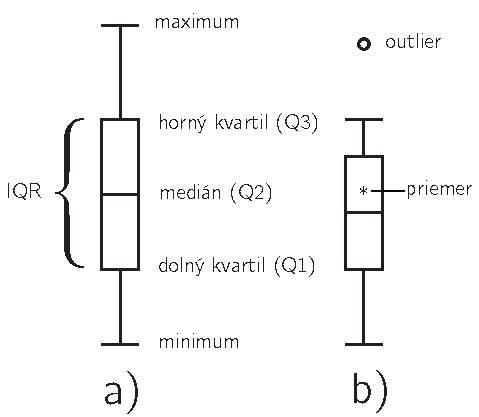
\includegraphics[width = 3.5in]{boxplot}
	\caption{Pôvodný návrh krabicového diagramu, ako bol prezentovaný v práci \textit{Exploratory Data Analysis}(1977) \cite{Tukey} }
	\label{fig:boxplot}
\end{figure}


\subsubsection{Ďalšie variácie krabicového diagramu}

Popularita krabicového diagramu nevyhnutne viedla k jeho vývoji a modifikáciám. Môžeme hovoriť o dvoch druhoch modifikácií. Jednak \textit{syntaktickej} (vizuálnej), kedy sa zachovávajú všetky vlastnosti a informácie ako v pôvodnom diagrame, len sa menia vizuálne prvky grafu. A modifikácii \textit{sémantickej} pridaním ďalšej popisnej informácie do grafu, čo má na záver vplyv aj na jeho vizuálnu stránku.


\begin{figure}
	\centering
	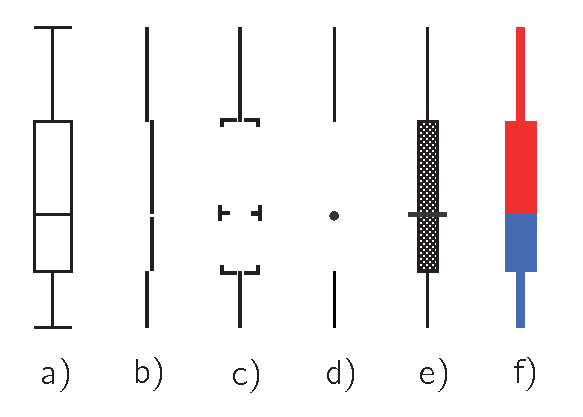
\includegraphics[width = 4in]{boxplot2}
	\caption{ a) Klasický krabicový diagram  b-f) Vizuálne variácie krabicového diagramu b-c) 2 variácie pre kvartilový graf \cite{Tufte83} c) Skrátený krabicový diagram \cite{VisualSummaryPotter} e) Range-bar chart \cite{Spear} f) Farebná variácia \cite{Carr}  }
	\label{fig:boxplotmodif1}
\end{figure}


\paragraph{}
{\large \textbf{\textit{N}}}a obrázkoch \ref{fig:boxplotmodif1} b-f) môžme vidieť niektoré vizuálne variácie krabicového diagramu. Vznik prvých troch motivovala snaha maximalizovať takzvaný \textit{data-ink} \cite{Tufte83}, teda množstvo atramentu alebo počet pixlov, ktoré zodpovedajú nejakým dátam. Autori sa teda snažili čo najviac znížiť počet vizuálnych prvkov a ponechať len tie, ktoré skutočne nesú nejakú informáciu. 

Na obrázku \ref{fig:boxplotmodif1} b) a c) vidíme dve z viacero riešení navrhnutých v knihe \textit{The Visual Display of Quantitative} \cite{Tufte83}, ktoré autor nazýva \textit{kvartilový graf}. Preceptuálne štúdie \cite{Stock} však ukázali, že tieto variácie sú výrazne menej presné ako originálny návrh.

Návrh d) ukazuje skrátený krabicový diagram \cite{VisualSummaryPotter}, ktorý sa taktiež snažil zredukovať množstvo okupovaného vizuálneho priestoru. Rozdielom je však to, že jeho účelom nie je existovať samostatne, ale ako súčasť \textit{summary plot}-u, ktorý zahŕňa histogram a ďalšie glify znázorňujúce informácie ako priemer, štandardná odchylka alebo koeficient asymetrie.

Obrázok \ref{fig:boxplotmodif1} e) znázorňuje predchodcu krabicového diagramu \textit{range} graf alebo tiež nazývaný \textit{range-bar} graf, ktorého autorkou je Mary Eleanor Spear \cite{Spear}.

Ako posledný príklad vizuálnej modifikácie uvádzame pridanie farieb do krabicového diagramu. Táto farebná variácia uchováva tvar diagramu, avšak časť nad mediánom je zafarbená inou farbou ako hodnoty pod. Autori článku odporúčajú červenú a modrú farbu, tak ako na obrázku \ref{fig:boxplotmodif1} f). Cieľom tohto prístupu bolo chápať krabicový diagram ako jednu percepčnú jednotku a nahradiť 5 symbolov jedným, čím sa mala znížiť námaha pozorovateľa pri analýze a taktiež uľahčiť porovnávanie viacerých diagramov navzájom. 


\begin{figure}
	\centering
	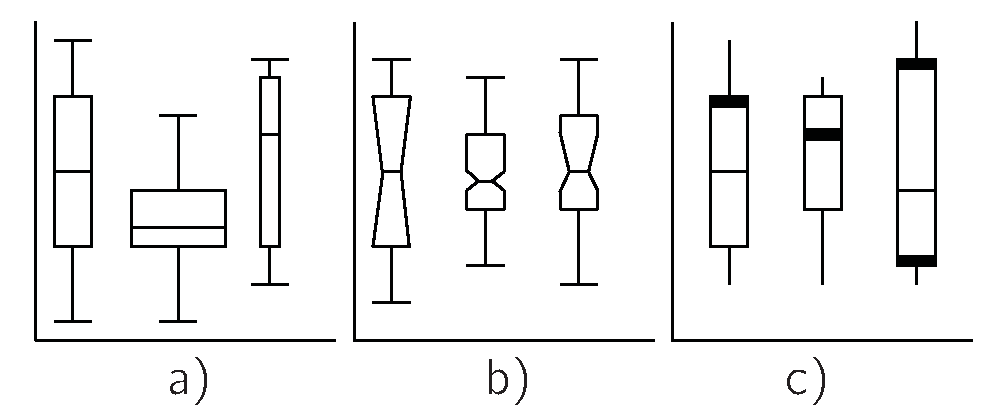
\includegraphics[width = 6in]{boxplot3}
	\caption{Krabicové diagramy s pridanou informáciou a) Krabicový diagram s variabilnou šírkou \cite{McGill} b) Vrúbkovaný krabicový diagram \cite{McGill} c) Krabicový diagram s informáciou o šikmosti dát \cite{Chamnein}}
	\label{fig:boxplotmodif2}
\end{figure}


\paragraph{}
{\large \textbf{\textit{K}}}rabicový diagram umožňuje svojim vzhľadom zakódovanie ďalšej informácie do grafu. Na obrázku \ref{fig:boxplotmodif2} vidíme aspoň niektoré najčastejšie úpravy... %TODO finish this sentence

Len rok po oficiálnom publikovaní krabicového diagramu vznikol článok \cite{McGill}, ktorý zhŕňa jeho tri najčastejšie používané modifikácie, z ktorých prvé dve môžme vidieť na obrázkoch \ref{fig:boxplotmodif2}a) a \ref{fig:boxplotmodif2}b) a tretí je ich kombináciou. V prvom prípade sa využíva šírka boxu na zakódovanie veľkosti množiny, ktorú skrýva za sebou diagram. Takýto graf sa nazýva \textit{Krabicový diagram s variabilnou šírkou}.  
V druhom prípade ide o takzvaný \textit{Vrúbkovaný krabicový diagram}. V tomto grafe sú pridané \textit{vrúbky}, ktoré zhruba naznačujú ako výrazné sú rozdiely v miere spoľahlivosti rôznych dátových množín. 

V niektorých prípadoch krabicový diagram zakrýva skutočný tvar dát, teda jeho šikmosť alebo modalitu, keďže jeho vzhľad nabáda k tomu, aby si užívateľ myslel, že sú dát zacentrované na stred a unimodálne. V práci s názvom \textit{Can the Box Plot be Improved?} \cite{Chamnein} autor uvádza príklad kedy skutočne rôznorodé dáta generujú rovnaký krabicový diagram. Tento problém rieši elegantným a čistým spôsobom pridaním hrubej čiary na základe koeficientu asymetrickosti $ \gamma $. Na obrázku \ref{fig:boxplotmodif2}c) môžme vidieť zľava asymetrické dáta, na stred zarovnané dáta a bimodálne dáta.

%TODO toho pottera mozem nahradit tymi, ktory su origos autori
Krabicový diagram umožňuje mnoho ďalších rozšírení napríklad pridaním informácie o hustote dát (histogramový krabicový diagram, vázový diagram \cite{HistVasePlot} , huslový diagram \cite{ViolinPlot}), rozšírením pre viacrozmerné dáta (vrecový graf \cite{Bagplot}, 2D krabicový diagram \cite{Boxplot2D} ) alebo zobrazením hodnôt v inej súradnicovej sústave (napríklad polárnej - vejárový graf \cite{FanChart}). Opis týchto techník je však nad rámec tejto práce, preto ho tu ani nebudeme uvádzať.

\subsubsection{Úloha krabicového diagramu vo verifikácii}

Ako sme spomenuli v úvode tejto sekcie, vo všeobecnosti je úlohou krabicového diagramu zobraziť distribúciu dát v kompaktnom tvare a teda slúži na rýchle porovnanie distribúcií viacerých skupín dát.
Pri verifikácii spojitej predpovede sa používa na viacero účelov a my tu spomenieme len niekoľko z nich. 

V prvom rade ide o porovnanie distribúcie predpovedí s distribúciou pozorovaní za istý časový interval. V takomto prípade máme vedľa seba iba dva krabicové diagramy, ktoré navzájom porovnávame. Použitie krabicového diagramu v takomto prípade, kedy jeden graf pozostáva iba z niekoľkých (2 až 4) krabicových diagramov považujeme za zbytočné. Pri takomto počte nie je potreba na redukciu vizuálnych prvkov a existujú lepšie techniky na vizualizáciu distribúcie, ktoré sprostredkúvajú viacej informácie a teda môže byť analýza efektívnejšia. 

Ďalším použitím je porovnanie distribúcie chýb predpovedí, či už pre rôzne merania, konkrétne predpovedané časy, rôzne predpovedné modely a podobne. Tu považujeme použitie krabicového diagramu za opodstatnené, keďže ide zväčša o porovnávanie väčšieho množstva distribúcií, a tak je jeho jednoduchosť, čitateľnosť, kompaktnosť a iné jeho vlastnosti potrebné.

\subsection{Time series plot}